\documentclass[10pt,a4paper]{article}
\usepackage[utf8]{inputenc}
\usepackage[english,russian]{babel}
\usepackage{cmap}
\usepackage[OT1]{fontenc}
\usepackage{amsmath}
\usepackage{amsfonts}
\usepackage{amssymb}
\usepackage{graphicx}
\usepackage{float}
\usepackage{wrapfig}
\usepackage{caption}
\DeclareCaptionLabelSeparator{dot}{. }
\captionsetup{justification=centering,labelsep=dot}
\graphicspath{{pictures/}}
\DeclareGraphicsExtensions{.pdf,.png,.jpg,.eps}
\begin{document}

\textbf{17	Исследование}\\

\textbf{17.1	Введение}\\

Эта глава посвящена задаче исследования с помощью роботов. Исследование – это задача управления роботом таким образом, чтобы максимизировать его осведомленность об окружающем его мире. Во многих отраслях робототехники роботы изначально предназначены для доставки информации нам, пользователям. Некоторые среды могут быть просто недоступны для людей, в других посылать людей может быть невыгодно, и роботы представляют собой самый наилучший способ сбора информации. Задача исследования является одной из основополагающих в робототехнике. Роботы исследуют заброшенные шахты, места радиоактивных выбросов, и даже Марс.

Задачи исследования могут быть самыми разнообразными. Например, целью робота может быть составление карты статической среды. Если представить среду с помощью карты сетки занятости, задача исследования является задачей максимизации общего количества информации по каждой ячейке.\\

ЗАДАЧА УХОДА ОТ ПРЕСЛЕДОВАНИЯ\\
Более динамичная версия задачи включает движущихся актеров: например, робот пытается найти в известной среде движущегося человека, как часть \textit{задачи ухода от преследования}. Целью может быть максимизация информации о местонахождении человека, а обнаружение человека может потребовать исследования среды. Однако, поскольку человек может двигаться, политикой исследования может быть предусмотрено повторное исследование областей несколько раз. Третья задача возникает, когда робот пытается определить своё местоположение в процессе локализации.\\

АКТИВНАЯ ЛОКАЛИЗАЦИЯ\\
Эта задача
обычно называется \textit{активной локализацией}, а ее целью является максимизация информации о собственном положении робота. При манипулировании предметами с помощью робота задача исследования возникает, когда перед манипулятором с датчиком возникает незнакомый предмет. Как показывает это короткое обсуждение, задачи исследования в робототехнике возникают практически повсеместно.

На первый взгляд, можно подумать, что задача исследования уже  полностью охвачена подходом POMDP, обсуждаемом в предыдущих главах. Как было показано, POMDP изначально ориентирован на сбор информации. Для превращения POMDP в алгоритм, единственной целью которого является максимизация информации, все, что нужно – это соответствующая функция дохода. Подходящим выбором является усиление информации, измеряющее уменьшение энтропии гипотезы робота в виде функции его действий. С такой функцией награды POMDP решает задачу исследования.

Однако, часто исследование с помощью алгоритма POMDP не такая уж хорошая идея. Это происходит потому, что во многих задачах количество неизвестных переменных состояния огромно, как и количество возможных измерений. Возьмём, для примера задачу исследования неизвестной планеты. Количество переменных, требуемых для описания поверхности планеты будет просто гигантским. Таким же будет и количество измерений, которые может совершить робот. Кака мы уже обнаружили, в общем алгоритме POMDP сложность планирования возрастает дважды экспоненциально относительно количества измерений (в худшем случае), и вычисление функции дохода просто невозможно. Фактически при столь огромном количестве \textit{возможных} значений для неизвестных переменных состояния в исследовании, любой алгоритм, выполняющий интегрирование по всем возможным значениям, в конце концов, станет непригодным для задач исследования высокой размерности просто по причинам вычислительной сложности.

В этой главе описано семейство практических алгоритмов, способных решать проблемы исследования высокой размерности. Все обсуждаемые методы являются \textit{жадными}. Другими словами, их горизонт ограничен следующим действием исследования. Однако, действие исследования может включать последовательность действий управления.\\

ДЕЙСТВИЕ ИССЛЕДОВАНИЯ\\
Например, будут обсуждаться алгоритмы, выбирающие местоположение для исследования на всей карте, при этом передвижение к точке считается одним \textit{действием управления}. Обсуждаемые алгоритмы также аппроксимируют усиление информации из восприятия, в целях уменьшения вычислительных затрат.

Изложение организовано следующим образом\\

•	Начнём с общего определения усиления информации в исследовании для дискретного и непрерывного случаев. Определим общий жадный алгоритм исследования, выбирающий действия так, чтобы максимизировать усиление информации.\\

•	Затем проанализируем первый особый случай исследования с помощью робота: \textit{активную локализацию}. При активной локализации выбор действий выполняется во время глобальной локализации робота. Применение такого жадного алгоритма исследования при соответствующем определении пространства действий,  даст практический способ решения задачи.\\ 

•	Также рассмотрим задачу исследования в построении сеток занятости. Мы выведем популярный метод, называемый \textit{исследованием на основе границ (frontier-based exploration)}, в котором робот двигается в направлении ближайшей границы.\\

•	Далее будет описано обобщение алгоритма исследования для систем из нескольких роботов и показано, каким образом можно управлять группой мобильных роботов для эффективного исследования неизвестной среды.\\

•	Наконец, рассмотрим приложение методов исследования к задаче SLAM. На примере FastSLAM будет показано, каким образом можно управлять роботом, чтобы минимизировать неопределённость в SLAM.\\

Описанные ниже методы исследования широко освещены в литературе и используются во множестве практических реализаций. Они также применимы для большого количества различных выражений и задач робототехники.\\

\textbf{17.2	Основные алгоритмы исследования}\\

\textbf{17.2.1	Прирост информации}\\

Информация – ключ к исследованию. Мы уже сталкивались с разнообразным использованием информации в вероятностной робототехнике.\\

ОЖИДАЕМАЯ ИФОРМАЦИЯ\\
В контексте исследования
определим энтропию $H_p(x)$ вероятностного распределения $p$ как ожидаемую
информацию $E[- \log p]$\\

(17.1)
$$H_p(x)=-\int p(x)\log p(x)dx\hspace{5mm}\text{или}\hspace{5mm}-\sum_xp(x)\log p(x)$$

Энтропия уже кратко обсуждалась в разделе 2.2. Значение $H_p(x)$ максимально, если $p$ представляет собой равномерное распределение. Она достигает минимума, когда $p$ – точечное распределение. Однако, в некоторых непрерывных случаях, например, гауссовских, можно никогда не достичь полной уверенности.\\

УСЛОВНАЯ ЭНТРОПИЯ\\

Условная энтропия определяется как энтропия условного распределения.
В исследовании мы стремимся минимизировать ожидаемую энтропию гипотезы после выполнения действия, потому, что она естественным образом зависит от измерения $z$ и управляющего воздействия $u$, которое определяет переход состояния гипотезы.

Придерживаясь приведённой выше записи, обозначим $B(b, z, u)$ гипотезу после выполнения управляющего действия $u$ и наблюдения $z$ при имеющейся гипотезе $b$. Условная энтропия состояния $x'$ после выполнения управляющего действия $u$ и измерения $z$ задана как\\

(17.2)
$$H_b(x'|z,u)=-\int B(b,z,u)(x')\log B(b,z,u)(x')dx'$$

Здесь $B(b, z, u)$ вычисляются, используя байесовский фильтр. В робототехнике выбор имеется только для управляющего действия $u$, а выбрать измерение $z$ невозможно. Следовательно, во внимание принимается только условная энтропия управления $u$, а измерения отбрасываются:\\

(17.3)
\begin{equation*}
\begin{split}
H_b(x'|u)&\approx E_z[H_b(x'|z,u)]\\
&=\iint H_b(x'|z,u)p(z|x')p(x'|u,x)b(x)dz\,dx'\,dx
\end{split}
\end{equation*}

ПРИРОСТ ИНФОРМАЦИИ\\

Заметим, что это лишь приближение, поскольку в финальном выражении порядок суммирования и логарифмирования обратный. \textit{Прирост информации} связанный с действием $u$ гипотезы $b$ задан разницей\\

(17.4)
$$I_b(u)=H_p(x)-E_z[H_b(x'|z,u)]$$

\textbf{17.2.2	Жадные методы}\\

Планируемый прирост информации позволяет перефразировать задачу исследования как теоретическую проблему принятия решений похожую на рассматриваемые в предыдущих главах. В частности, пусть $r(x, u)$ будет стоимостью применения управляющего действия $u$ в состоянии $x$. Здесь будем считать, что $r(x, u)<0$ для сохранения целостности описания. Тогда оптимальное жадное исследование для гипотезы $b$ максимизирует разницу между приростом информации и стоимостью, взвешенной коэффициентом $\alpha$.\\

(17.5)
$$\pi(b)=\underset{u}{\text{argmax}}\,\alpha\,\underbrace{(H_p(x)-E_z[H_b(x'|z,u)])}_{\text{expected information gain}}+\underbrace{\int r(x,u)b(x)dx}_{\text{expected costs}}$$

Коэффициент $\alpha$ соотносит информацию и стоимость выполнения действия $u$. Он определяет ценность информации для робота, а также цену, которую алгоритм готов платить в смысле стоимости получения информации.

Выражение (17.5) разрешается как\\

(17.6)
\begin{equation*}
\begin{split}
\pi(b)&=\underset{u}{\text{argmax}}-\alpha\,E_z[H_b(x'|z,u)]+\int r(x,u)\,b(x)\,dx\\
&=\underset{u}{\text{argmax}}\int[r(x,u)-\alpha\iint H_b(x'|z,u)p(z|x')p(x'|u,x)dz\,dx']\,b(x)\,dx
\end{split}
\end{equation*}

В двух словах, для понимания полезности управляющего действия $u$ требуется вычислить ожидаемую энтропию после выполнения $u$ и наблюдения. Ожидаемая энтропия получается интегрированием по всем возможным измерениям $z$, которые может получить робот, умноженным на их вероятность.  Она транслируется в показатель полезности с помощью константы $\alpha$. Затем вычитается ожидаемая стоимость выполнения действия $r$.

\begin{figure}[H]
	\center{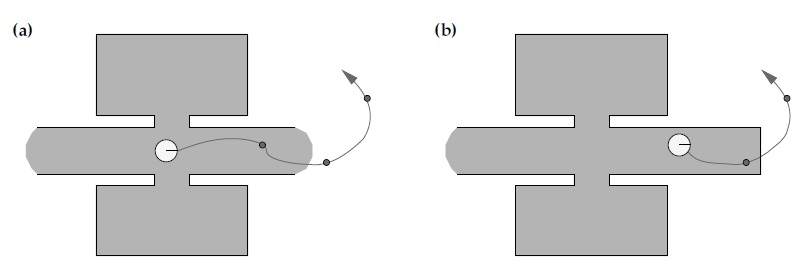
\includegraphics[width=1\linewidth]{171orig}}
	\caption{ ( Рис. 17.1 Непредсказуемость задачи исследования: Робот на схеме (a) может выполнить последовательность трёх управляющих действий, но их исполнимость зависит от ситуации, которую ему только предстоит обнаружить на пути. Любая политика исследования должна иметь возможность реагировать различными способами.) }
	\label{fig:171orig}
\end{figure}

В большинстве методов исследования используется подобная жадная политика, которая, действительно, оптимальна для горизонта 1. Причина такой приверженности жадным методам состоит в чудовищном количестве разветвлений в процессе исследования, что делает планирование на несколько шагов вперёд невозможным. Коэффициент разветвления так велик в силу самой природы проблемы исследования, ведь его целью является получение новой информации, но как только информация была получена, робот оказывается с новой гипотезой состояния, и вынужден перестраивать политику. Поэтому, измерения изначально непредсказуемы.

На Рис. 17.1 показана такая ситуация. Здесь робот выполнил картографирования двух комнат и части коридора. В этой точке оптимальное исследование может включать исследование коридора, а соответствующая последовательность действий может совпадать с показанной на Рис. 17.1a. Однако, исполнима эта последовательность или нет – остаётся совершенно непредсказуемым. Например, робот может обнаружить, что оказался в тупике, как показано на Рис. 17.1b, и выбранная последовательность действий неприменима.\\

\textbf{17.2.3	Исследование методом Монте-Карло}\\

Алгоритм \textbf{Monte\_Carlo\_exploration} – это простой вероятностный алгоритм исследования. В Таблице 17.1 приводится аппроксимация жадного алгоритма исследования в выражении (17.6) методом Монте-Карло. Этот алгоритм просто заменяет интегралы в жадном методе выборкой. В строке 4  выполняется выборка состояния $x$ из текущей гипотезы $b$, за которой следует выборка следующего состояния $x'$ и соответствующее наблюдение $z'$. Затем новая апостериорная гипотеза вычисляется в строке 8, а компромисс энтропия-стоимость кэшируется в строке 9. В строке 12 возвращается действие, с наибольшей величиной «прирост показателя информация-стоимость» по методу Монте-Карло.

\begin{table}[H]
\begin{center}
\begin{tabular}{|l|}
\hline
{}\\
1:\textbf{ Algorithm Monte\_Carlo\_exploration}$(b):\qquad\qquad\qquad$\\
2:\hspace{5mm}$\textit{установить}\,\,\rho_u=0\,\,\textit{для всех действий u}$\\
3:\hspace{5mm}$\textit{for}\,\,i=1\,\,\textit{to}\,\,N\,\,\textit{do}$\\
4:\hspace{10mm}$\textit{выборка}\,\,x\sim b(x)$\\
5:\hspace{10mm}$\textit{для всех действий управления u выполнить}$\\
6:\hspace{15mm}$\textit{выборка}\,\,x'\sim p(x'|u,x)$\\
7:\hspace{15mm}$\textit{выборка}\,\,z\sim p(z|x')$\\
8:\hspace{15mm}$b'=\textbf{Bayes\_filter}\,(b,z,u)$\\
9:\hspace{15mm}$\rho_u=\rho_u+r(x,u)-\alpha H_{b'}(x')$\\
10:\hspace{9mm}$\textit{endfor}$\\
11:\hspace{4mm}$\textit{endfor}$\\
12:\hspace{5mm}$\textit{return}\,\,\underset{u}{\text{argmax}}\,\,\rho_u$\\
{}\\
\hline
\end{tabular}
\caption{(Таблица 17.1 Реализация жадного алгоритма исследования методом Монте-Карло. Действия выбираются максимизацией компромисса между приростом информации и стоимостью.)}
\end{center}
\end{table}

В общем случае жадный алгоритм Монте-Карло все ещё может требовать значительного времени на выполнение, что может привести к невозможности использования. Основная сложность возникает при выполнении выборки измерений $z$. При исследовании неизвестной среды в процессе картографирования количество возможных измерений может быть огромным. Например, для робота, оборудованного 24 ультразвуковыми датчиками, каждый из которых передаёт один байт данных расстояния, количество потенциальных сканирований сонара, полученных в конкретном местоположении, составляет $256^{24}$. Очевидно, не все эти измерения применимы, но количество применимых измерений, по меньшей мере, так же велико, как число применимых локальных карт. А для любой реалистичной проблемы картографирования количество возможных карт просто беспредельно! Ниже будут обсуждаться методы исследования, которые обходят это интегрирование с помощью анализа ожидаемого прироста информации в закрытой форме.\\

\textbf{17.2.4	Многоступенчатые методы}

В ситуациях, когда пространства состояний и измерений ограничены, может оказаться возможным обобщить принцип сбора информации для произвольного коечного горизонта $T>1$. Допустим, необходимо оптимизировать баланс между приростом информации и стоимостью для горизонта $T$. Это можно выполнить, определив следующую функцию дохода при исследовании:\\

(17.7)
\begin{equation*}
r_{\exp}(b_t,u_t)= \left\{
\begin{array}{ll}
\int r(x_t,u_t)b(x_t)dx_t& \mbox{ при } t < T \\
\alpha\,H_{b_t}(x_t)& \mbox{ при } t = T
\end{array}
\right.
\end{equation*}

Для этой функции планировщик POMDP находит политику управления, которая минимизирует энтропию финальной гипотезы $b_T$ за вычетом стоимости достижения этой гипотезы в соответствующем масштабе. В данном случае применимы все обсуждаемые методы POMDP.

Читатель может заметить сходство с дополненным алгоритма MDP, обсуждаемом в предыдущей главе. Разница состоит в том, что здесь определяется только функция дохода, но не выражение гипотез состояния. Поскольку большинство задач исследования становятся вычислительно невыполнимыми для общей модели POMDP, этот подход далее обсуждаться не будет.\\

\textbf{17.3	Активная локализация}\\

Простейший случай исследования происходит при оценке состояния переменной с низкой размерностью. Такой задачей является \textit{активная локализация}: здесь выполняется поиск информации о положении робота $x_t$, но дана карта среды. Активная локализация особенно интересна при глобальной локализации, поскольку в ней выбор управления может иметь огромное воздействие на прирост информации. Во многих средах бесцельное перемещение по окрестностям затрудняет глобальную локализацию, а передвижение к верному местоположению позволяет выполнить ее очень быстро.

Такая среда показана на Рис. 17.2a. Здесь робот помещается в симметричный коридор, что делает невозможным определение положения сколь долго он перемещается по нему. Единственным способом оказывается действия ухода из коридора через одну из открытых дверей. Таким образом, любое решение задачи активной локализации должно обязательно направить робота из коридора в одну из комнат.

\begin{figure}[H]
	\center{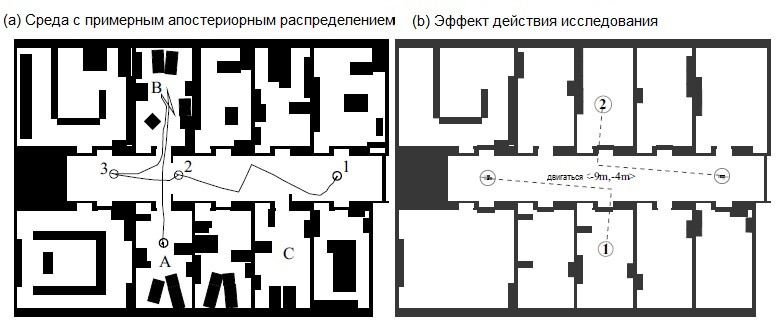
\includegraphics[width=1\linewidth]{172orig}}
	\caption{ ( Рис. 17.2  Активная локализация в симметричной среде: Здесь показана среда с симметричным коридором, но ассиметричной обстановкой комнат, обозначенных A, B и C. На рисунке также показан путь исследования(a).  Пример действия исследования «пройти назад 9 метров, налево 4 метра». Если апостериорное положение робота имеет две различимые моды, как показано на картинке, выполнение управляющего действия в глобальных координатах среды может привести в два разных места.(b)) }
	\label{fig:172orig}
\end{figure}

Активная локализация может быть решена жадным методом с помощью только что представленного алгоритма. Ключевой идеей является выбор выражения действия. Очевидно, что, если действия определять как низкоуровневые, как в большей части книги, любой разумный план разрешения неопределенности положения путём исследования будет состоять из длинной цепочки управляющих действий. Для решения задачи активной локализации с помощью жадного исследования требуется определение действий, с помощью которых робот способен выполнять сбор информации.

Одним из возможных решений является определение \textit{действия исследования} через целевые местоположения, выраженные в локальной системе отсчёта робота. Например, действием может считаться \textit{“двигаться в точку }$\varDelta x = -9$ \textit{м и}  $\varDelta y = 4$ \textit{м относительно текущего местоположения в локальной системе отсчёта”}, до тех пор, пока имеется низкоуровневый модуль навигации, способный проецировать это действие в низкоуровневые сигналы управления. На Рис. 17.2b показан потенциальный эффект такого действия в глобальной системе координат. В этом примере апостериорное распределение имеет две моды, поэтому действие может перенести робота в два разных местоположения.

Определение действий относительного передвижения позволяет решить задачу активной локализации с помощью алгоритма, практически аналогичного жадному алгоритму исследования в Таблице 17.1. Опишем его на примере. На Рис. 17.3a показан путь активной локализации и несколько помеченных местоположений. Начнём с середины: на Рис. 17.3b показана гипотеза после передвижения из местоположения, отмеченного “1” в местоположение с меткой “2”. В этой гипотезе имеется шесть мод, каждая обозначена кружком на Рис. 17.3b. Для этой гипотезы ожидаемая занятость  по координатам робота показана на Рис. 17.3c. Этот рисунок получен сложением известной карты сетки занятости для каждого из положений робота, взвешенных соответствующими вероятностями. Поскольку робот не имеет чёткого понимания своего положения, знать занятости местоположений он не может, отсюда и «нечёткость» карты ожидаемой стоимости. Однако, с большой вероятностью робот находится в зоне, напоминающей коридор, и она проходима.

Хотя на Рис. 17.3c показана стоимость \textit{нахождения} в целевом местоположении, необходима стоимость \textit{передвижения} в такое целевое местоположение. Алгоритм для вычисления такой стоимости передвижения уже приводился, как и вычисление оптимального пути: \textit{итерация согласно критерию} (см. Главу 14). На Рис. 17.3d показан результат итерационного алгоритма, применённый к карте на Рис. 17.3b в виде функции стоимости. Здесь значение распространяется от робота (противоположно цели, как было в записи в Главе 14). Это делает возможным вычисление стоимости передвижения в \textit{любую} потенциальную целевую точку карты.

Как показано на рисунке, существует большая зона около робота, где перемещение безопасно. Фактически, эта область соответствует коридору, вне зависимости от того, где действительно находится робот. Перемещение за границы этой области и в одну из комнат имеет более высокую ожидаемую стоимость, поскольку применимость такого движения основана на знании точного местоположения робота, которое неизвестно.

\begin{figure}[H]
	\center{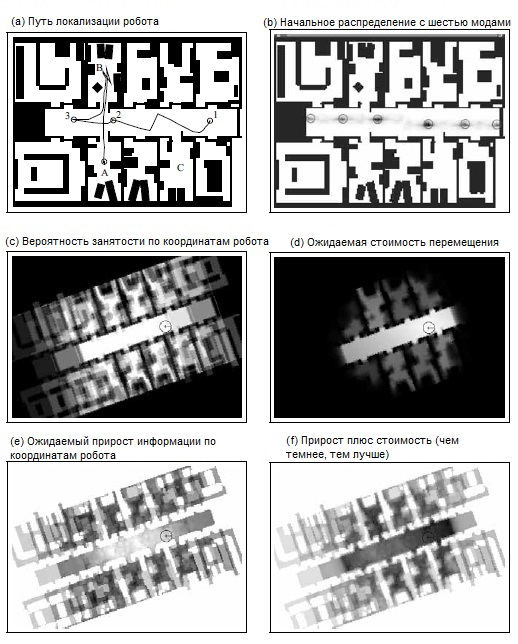
\includegraphics[width=1\linewidth]{173orig}}
	\caption{ ( Рис. 17.3 Иллюстрация активной локализации. На рисунке показаны несколько вспомогательных функций для вычисления оптимального действия в распределении положений с несколькими гипотезами. ) }
	\label{fig:173orig}
\end{figure}

\begin{figure}[H]
	\center{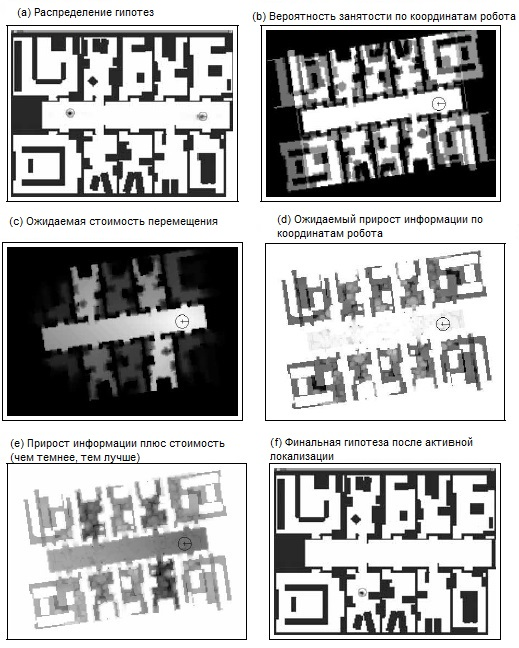
\includegraphics[width=1\linewidth]{174orig}}
	\caption{ ( Рис. 17.4 Иллюстрация активной локализации в более поздний момент времени для гипотезы с двумя выраженными модами.) }
	\label{fig:174orig}
\end{figure}

Для жадного исследования теперь требуется определить ожидаемый прирост информации. Его можно аппроксимировать, поместив робота в какое-либо положение, смоделировав возможные измерения расстояния, учтя результат, и измерив количество информации после байесовского обновления. Повторение этого этапа оценки для каждого возможного местоположения даст карту ожидаемого прироста информации. На Рис. 17.3e показан результат: чем темнее местоположение на карте, тем больше информации оно предоставляет, относительно оценки положения робота. Очевидно, любая из комнат будет наиболее информативна, по сравнению с торцами коридора. Поэтому, исходя их чистой перспективы прироста информации, роботу необходимо искать возможность переместиться в одну из комнат.

Добавление карты стоимости к ожидаемому приросту информации даст график на Рис. 17.3f: чем темнее целевое местоположение, тем лучше. Хотя показатели внешних комнат для комбинированной функции тоже высоки, их полезность уменьшена относительно высокой стоимостью передвижения в них. В этой точке, местоположения в концах коридора имеют наибольшую полезность.

Теперь робот перемещается в местоположение с наивысшим комбинированным значением, что приводит его во внешнюю часть коридора, куда все ещё безопасно перемещаться. На Рис. 17.3a, это соответствует перемещению из местоположения, отмеченного “2”, к  точке, отмеченной “3”.

Выполняется следующая итерация жадного алгоритма исследования с помощью активной локализации. Гипотеза в местоположении “3” показана на Рис. 17.4a. Очевидно, предыдущее действие исследования позволило сократить количество мод апостериорного распределения с шести до двух. На Рис. 17.4b показана новая карта занятости в локальных координатах робота. На Рис. 17.4c показана соответствующая функция дохода. Ожидаемый прирост информации теперь равномерно высок только в комнатах, как показано на Рис. 17.4d. На Рис. 17.4e приведена комбинированная карта прироста стоимости. В этой точке стоимость передвижения в любую из симметричных открытых комнат самая низкая, поскольку робот переместился в точку, в которой неопределённость положения, по большей части, разрешена. Финальная гипотеза После ещё одного шага и ещё одного уточнения показана на Рис. 17.4f.

Этот жадный алгоритм активной локализации имеет и недостатки. Первый недостаток возникает в силу самого подхода на основе жадности, поскольку он неспособен объединять несколько действий исследования, которые вместе максимизируют прирост информации. Другой недостаток – результат определения действия. Алгоритм не может учитывать измерения, которые будут получены на пути к целевому местоположению. Вместо этого, каждое такое действие воспринимается как открытый цикл, в котором робот неспособен реагировать на измерения. Конечно, встретив закрытую дверь, настоящий робот может отменить целевую точку даже до момента ее достижения. Однако при планировании этого не делается. Этим объясняется почти оптимальный выбор в примере выше, где робот исследует комнату, отмеченную “B” до того, как исследует комнату с меткой “A.” В результате, локализация занимает больше времени, чем это, теоретически, необходимо. В любом случае, алгоритм хорошо работает на практике.\\

\textbf{17.3	Исследование для обучающихся карт сетки занятости}\\

\textbf{17.3.1	Вычисление прироста информации}\\

Жадное исследование может также использоваться в картографировании с помощью роботов. Задачи построения карт включают намного больше неизвестных переменных, чем локализация робота, поскольку требуется метод вычисления ожидаемого прироста информации, масштабируемый для задач оценки высокой размерности. Как мы увидим, «хитрость» для карт сеток занятости ровно такая же, что привела к определению эффективного алгоритма обновления для карт сетки занятости. Нужно считать, что прирост информации между разными ячейками сетки \textit{независим}.

\begin{figure}[H]
	\center{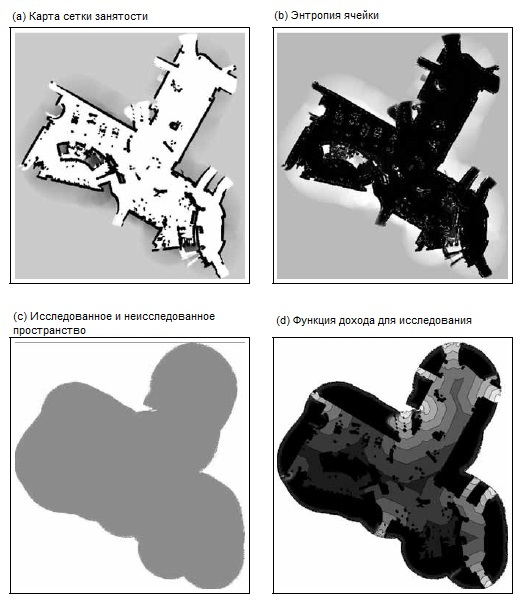
\includegraphics[width=1\linewidth]{175orig}}
	\caption{ ( Рис. 17.5 Пример важных шагов в исследовании для построения карт. Показана частичная карта сетки(a), показана энтропия карты (b),  показано пространство, для которой информация нулевая (c), и показана функция ценности для оптимального исследования(d). ) }
	\label{fig:175orig}
\end{figure}

\begin{figure}[H]
	\center{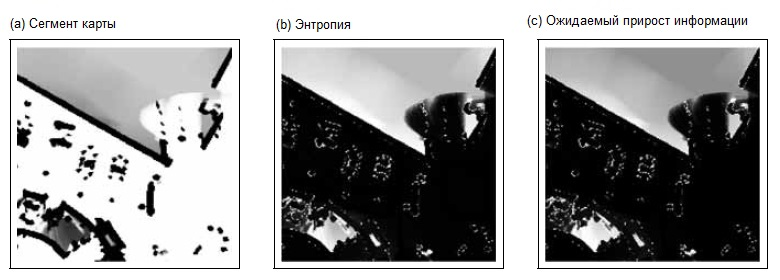
\includegraphics[width=1\linewidth]{176orig}}
	\caption{ ( Рис. 17.6 Карта, энтропия и ожидаемый прирост информации.  На рисунке показано соответствующее масштабирование, энтропия и ожидаемый прирост информации почти неразличимы.) }
	\label{fig:176orig}
\end{figure}

Возьмём карту сетки занятости, наподобие показанной на Рис. 17.5a. Некоторые части этой карты хорошо исследованы, например, большая свободная зона в центре карты и многие стены и препятствия, расположение которых хорошо известно. Другие части остаются не исследованными, например, большая серая зона за пределами карты. Жадное исследование направляет робота к ближайшей неисследованной зоне, где прирост информации максимален. Это поднимает вопрос о способе вычисления прироста информации. 

Обсудим три возможных метода. Все три подхода имеют общую черту, что вычисляется прирост информации \textit{для ячейки сети}, а не функцию действия робота. Это даёт карту прироста информации, которая представляет собой двухмерную карту, определённую по той же сетке, что и оригинальная сетка карты. Разница между этими методами состоит в качестве аппроксимации.\\

•\textbf{	Энтропия.} Вычисление энтропии для каждой ячейки очевидно. Обозначим $i$-ю ячейку как $m_i$, а вероятность занятости $p_i = p(m_i)$. Тогда энтропия бинарной переменной занятости задана следующей суммой:\\

(17.8)
$$H_p(\textbf{m}_i)=-p_i\log p_i-(1-p_i)\log(1-p_i)$$

На Рис. 17.5b показана энтропия для каждой из ячеек на карте, показанной на Рис. 17.5a. Чем светлее местоположение, тем выше энтропия. Большая часть центральных областей карты показывается с низкой энтропией, за исключением нескольких зон около или внутри препятствий. Это соответствует интуитивному пониманию, так как большая часть карты уже хорошо изучена. Энтропия внешних областей высокая, что указывает на высокую пригодность для исследования. Поэтому, карта энтропии назначает высокие значения ценности для мест, которые остались неисследованными.\\

•	Ожидаемый прирост информации. Технически, энтропия способна измерить только текущую информацию. Она не обозначает информацию, которую робот может получить с помощью датчиков, в непосредственной видимости от ячейки. Вычисление ожидаемого прироста информации чуть более сложно, и требует дополнительных допущений относительно природы информации, приходящей с датчиков робота.

Допустим, датчик даёт измерение верной занятости с вероятностью $p_{true}$, и ошибается с вероятностью $1-p_{true}$. Тогда можно ожидать измерения «занято» со следующей вероятностью:\\

(17.9)
$$p^+=p_{true}p_i+(1-p_{true})(1-p_i)$$

стандартное обновление сетки занятости даст новую вероятность, которая напрямую следует из алгоритма картографирования сетки занятости, обсуждаемого в Главе 9:\\

(17.10)
$$p_i'=\frac{p_{true}p_i}{p_{true}p_i+(1-p_{true})(1-p_i)}$$

Теперь энтропия апостериорного распределения:\\

(17.11)
\begin{equation*}
\begin{split}
H_{p'}^+(\textbf{m}_i)&=-\frac{p_{true}p_i}{p_{true}p_i+(1-p_{true})(1-p_i)}\log\frac{p_{true}p_i}{p_{true}p_i+(1-p_{true})(1-p_i)}\\
&-\frac{(1-p_{true})(1-p_i)}{p_{true}p_i+(1-p_{true})(1-p_i)}\log\frac{(1-p_{true})(1-p_i)}{p_{true}p_i+(1-p_{true})(1-p_i)}
\end{split}
\end{equation*}

По аналогии, датчик покажет «свободно» с вероятностью\\

(17.12)
$$p^-=p_{true}(1-p_i)+(1-p_{true})p_i$$

в этом случае апостериорное распределение станет\\

(17.13)
$$p_i'=\frac{(1-p_{true})p_i}{p_{true}(1-p_i)+(1-p_{true})p_i}$$

Это апостериорное распределение имеет энтропию\\

(17.14)
\begin{equation*}
\begin{split}
H_{p'}^-(\textbf{m}_i)&=-\frac{(1-p_{true})p_i}{p_{true}(1-p_i)+(1-p_{true})p_i}\log\frac{(1-p_{true})p_i}{p_{true}(1-p_i)+(1-p_{true})p_i}\\
&-\frac{p_{true}(1-p_i)}{p_{true}(1-p_i)+(1-p_{true})p_i}\log\frac{p_{true}(1-p_i)}{p_{true}(1-p_i)+(1-p_{true})p_i}
\end{split}
\end{equation*}

сводя все предыдущие выражения вместе, получим ожидаемую энтропию после обновления:\\

(17.15)
\begin{equation*}
\begin{split}
E[H_{p'}(\textbf{m}_i)]&=p^+H_{p'}^+(\textbf{m}_i)+p^-H_{p'}^-(\textbf{m}_i)\\
&=-p_{true}p_i\log\frac{p_{true}p_i}{p_{true}p_i+(1-p_{true})(1-p_i)}\\
&\hspace{4mm}-(1-p_{true})(1-p_i)\log\frac{(1-p_{true})(1-p_i)}{p_{true}p_i+(1-p_{true})(1-p_i)}\\
&\hspace{4mm}-(1-p_{true})p_i\log\frac{(1-p_{true})p_i}{p_{true}(1-p_i)+(1-p_{true})p_i}\\
&\hspace{4mm}-p_{true}(1-p_i)\log\frac{(1-p_{true})p_i}{p_{true}(1-p_i)+(1-p_{true})p_i}
\end{split}
\end{equation*}

Согласно определению в выражении (17.4), ожидаемый прирост информации после восприятия ячейки сетки $m_i$ - это просто разница $H_p(\textbf{m}_i)-E[H_{p'}(\textbf{m}_i)]$.\\

Так насколько лучше ожидаемый прирост информации, по сравнению с энтропией, из которой он был выведен? Ответ: ненамного. На Рис. 17.6 энтропия показана на схеме (b), рядом с ожидаемым приростом информации на схеме (c), все для сегмента карты, показанной на схеме (a). Визуально, энтропия и ожидаемый прирост информации почти неразличимы, хотя их значения различны. Это оправдывает общую практику использования энтропии как функции направления исследования вместо ожидаемого прироста информации.\\

•	Бинарный прирост. Третий метод самый простой из всех, и самый популярный. Очень грубая аппроксимация ожидаемого прироста информации отмечает ячейки, которые обновлялись, по меньшей мере, единожды, как «исследованные», а все остальные – «неисследованные». Таким образом, прирост становится бинарной функцией.\\

На Рис. 17.5c показана такая бинарная карта: только внешняя белая зона даст новую информацию. Внутренняя часть карты считается полностью исследованной. Хотя эта карта прироста информации, очевидно, самая грубая из всех обсуждаемых, на практике она хорошо работает, поскольку постоянно толкает робота вглубь неисследованной территории.\\
ИССЛЕДОВАНИЕ НА ОСНОВЕ ГРАНИЦ\\
Бинарная карта лежит в основе популярного метода исследования, который называется \textit{исследованием на основе границ},
когда робот постоянно двигается к ближайшей неисследованной границы исследованного пространства.\\

\textbf{17.3.2	Распространение прироста информации}\\

Оставшийся вопрос относится к разработке жадного метода исследования, использующего эти карты. Как и в примере активной локализации, это требует определения соответствующего действия исследования.

Простое, но эффективное определение \textit{действия исследования} включает передвижение в местоположение $x-y$ по пути с минимальной стоимостью, а затем восприятие по всем ячейкам сети на небольшом расстоянии по всем направлениям от робота. Таким образом, каждое местоположение на карте определяет потенциальное действие исследования.

Вычисление наилучшего жадного действия исследования теперь легко выполняется с помощью итерационного алгоритма. На Рис. 17.5d показана результирующая функция дохода для карты, показанной на Рис. 17.5a, а бинарная карта прироста информации для этой функции – на Рис. 17.5c. Итерационный алгоритм подразумевает такую бинарную сетку прироста, поскольку прирост может быть только в не обследованных местоположениях.

Центральное обновление значений выполняется с помощью следующей рекурсии:\\

(17.16)
\begin{equation*}
V_T(\textbf{m}_i) = \left\{
\begin{array}{cl}
\max_j\,r(\textbf{m}_i,\textbf{m}_j)+V_{T-1}(\textbf{m}_j)& \mbox{ при } I(\textbf{m}_i)=0 \\
I(\textbf{m}_i)& \mbox{ при } I(\textbf{m}_i) > 0
\end{array}
\right.
\end{equation*}

Здесь $V$ функция дохода, $j$ индексирует все значения ячеек с поправкой $\textbf{m}_i$, $r$, измеряя стоимость перемещения до точки (обычно функция карты сетки занятости), а $I(\textbf{m}_i)$ информацию, которую можно получить в ячейке $\textbf{m}_i$. Условие прекращения $I(\textbf{m}_i) > 0$ справедливо только для неисследованных ячеек на бинарной карте прироста информации.

На Рис. 17.5d показана такая функция ценности после сходимости. Здесь ценность наиболее высока в открытых частях карты, и ниже внутри карты. Метод исследования теперь просто определяет оптимальный путь методом поиска экстремума на карте. Этот путь приведёт робота к ближайшей неисследованной границе.

Очевидно, этот метод исследования является лишь грубой аппроксимацией. В нем полностью игнорируется информация, полученная робот при перемещении к целевому местоположению, и ошибочно считается, что робот при перемещении не воспринимает окружающее. Однако, он хорошо работает на практике. На Рис. 17.7 показана функция дохода и карта робота, выполняющего исследование. Это историческая карта: она была сделана на Соревновании мобильных роботов 1994 \textit{(1994 AAAI Mobile Robot Competition)}, которое включало получение карты окружающей среды с высокими скоростями. Робот был оборудован массивом из 24 ультразвуковых датчиков, подходящих для относительно низкой точности карты. Наиболее интересный аспект этой карты – траектория пути, пройденного роботом. Как видно на Рис. 17.7b, в начале исследование очень эффективно, и робот движется по неисследованным коридорам. Однако, позже робот начинает выбирать между различными целевыми локациями. Такое выборочное поведение характерно для жадных алгоритмов исследования, и самые современные реализации имеют дополнительные механизмы, которые позволяют избежать такого поведения.

\begin{figure}[H]
	\center{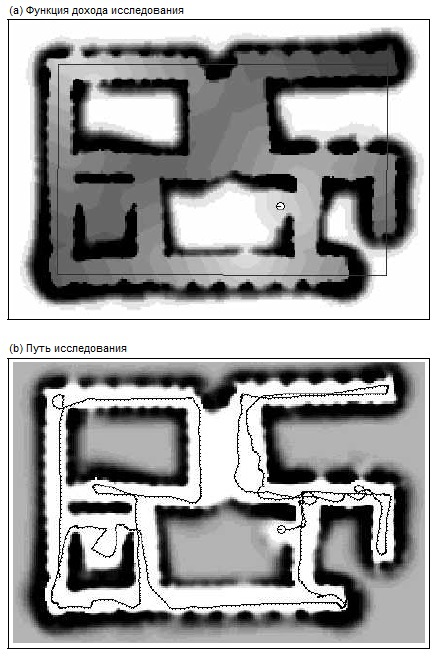
\includegraphics[width=0.95\linewidth]{177orig}}
	\caption{ ( Рис. 17.7 Иллюстрация автономного исследования. Значения дохода $V$ вычисляются с помощью итерации критерия. Белые области полностью не исследованы. Двигаясь по серому градиенту, робот двигается к следующему не открытому месту по пути с минимальной стоимостью. Большой чёрный прямоугольник обозначает глобальную ориентацию стен $\theta_{wall}$ (a). Текущий путь при выполнении исследования показана на схеме, вместе с результирующей метрической картой(b). ) }
	\label{fig:177orig}
\end{figure}

\begin{figure}[H]
	\center{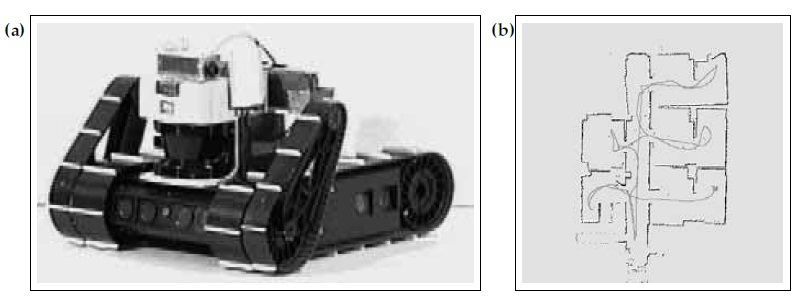
\includegraphics[width=1\linewidth]{178orig}}
	\caption{ ( Рис. 17.8  Городской робот для исследования внутри и вне помещений. Одометрия робота достаточно плохая(a). Путь исследования автономного исследовательского робота на основе методов, описанных в тексте.(b)) }
	\label{fig:178orig}
\end{figure}

Второй пример показан на Рис. 17.8. Путь робота, показанный справа, иллюстрирует эффективность жадного алгоритма исследования.\\

\textbf{17.3.3	Обобщение для систем нескольких роботов}\\

Правило исследования на основе прироста информации часто обобщается до системы из нескольких роботов, в которой роботы стремятся получить карту, используя исследование группой. В общем, ускорение от использования $K$ роботов линейное. Оно может быть и \textit{более, чем линейным}: $K$ роботов могут ускорять исследование больше, чем в $K$ раз по сравнению с одним роботом. Столь большое ускорение по сравнению с одним роботом вызвано тем, что один робот вынужден переходить через одни и те же места несколько раз - первый раз, чтобы пройти к месту исследования, и второй раз, чтобы вернуться для исследования другой части среды. При соответствующем количестве роботов, возвращение может оказаться ненужным, и степень ускорения будет близкой к $2K$. Коэффициент $2K$ является ограничением сверху для роботов, которые свободно передвигаются во всех направлениях.

Ключевым условием исследования с помощью нескольких роботов является координация действий. При статическом исследовании это легко достигается с помощью жадных методов распределения заданий. Рассмотрим ситуацию, в которой $K$ роботов помещены на частично исследованную карту. В данной ситуации существует несколько мест для исследования на границе и необходим алгоритм, назначающий роботам места, где исследование будет наиболее эффективно.

Алгоритм \textbf{multi\_robot\_exploration} в Таблице 17.2 является одним из простейших алгоритмов такого рода. Для набора из $K$ роботов вычисляется набор $K$ целей исследования в виде координат мест, куда роботы должны переместиться для исследования.

\begin{table}[H]
\begin{center}
\begin{tabular}{|l|}
\hline
{}\\
1:\textbf{ Algorithm multi\_robot\_exploration}$(m,x_1,...,x_K):\qquad\qquad\qquad$\\
2:\hspace{5mm}$\textit{для каждого робота }\,\,k=1\,\,\textit{до}\,\,K\,\,\textit{выполнить}$\\
3:\hspace{10mm}$\textit{Пусть}\,\,\textbf{m}_k\,\,\textit{будет ячейкой сетки для}\,\,x_k$\\
4:\hspace{10mm}
$V_k(\textbf{m}_i)=\left\{\begin{array}{ll}
\infty&\mbox{при}\textbf{m}_i\neq\textbf{m}_k\\
0&\mbox{при}\textbf{m}_i=\textbf{m}_k
\end{array}
\right.$
\\
5:\hspace{10mm}$\textit{выполнять до}\,\,V_k\,\,\textit{сходимости}$\\
6:\hspace{15mm}$\textit{для всех i выполнить}$\\
7:\hspace{20mm}$V_k(\textbf{m}_i)\longleftarrow\underset{j}{\min}\{V_k(\textbf{m}_i),r(\textbf{m}_i,\textbf{m}_j)+V_k(\textbf{m}_j)\}$\\
8:\hspace{15mm}$\textit{endfor}$\\
9:\hspace{10mm}$\textit{endwhile}$\\
10:\hspace{4mm}$\textit{endfor}$\\
11:\hspace{4mm}$\textit{вычислить бинарную карту прироста информации}\,\,\bar{m}\,\,\textit{из карты}\,\,m$\\
12:\hspace{4mm}$\textit{для каждого робота}\,\,k=1\,\,\textit{до}\,\,K\,\,\textit{выполнять}$\\
13:\hspace{9mm}$\textit{установить}\,\,\text{цель}_k=\underset{i\,\text{таким образом, что}\,\bar{\textbf{m}}_i=1}{\text{argmin}}V_k(\textbf{m}_i)$\\
14:\hspace{9mm}$\textit{для всех ячеек}\,\,\bar{\textbf{m}}_j\,\,\textit{in}\,\,\varepsilon-\textit{соседних с}\,\,\text{целью}_k$\\
15:\hspace{14mm}$\textit{установить}\,\,\bar{\textbf{m}}_j=0$\\
16:\hspace{9mm}$\textit{endfor}$\\
17:\hspace{4mm}$\textit{endfor}$\\
18:\hspace{4mm}$\textit{return}\,\,\{\text{цель}_1,\text{цель}_2,...,\text{цель}_K\}$\\
{}\\
\hline
\end{tabular}
\caption{(Таблица 17.2 Алгоритм исследования с помощью нескольких роботов.)}
\end{center}
\end{table}

Сначала алгоритм вычисляет значение функций дохода $V_k$, по одной для каждого робота (строки со 2 по 10). Однако, функции дохода теперь определяются не так, как было описано раньше:  минимальное значение назначается согласно положению робота. Чем дальше о него находится ячейка, тем выше значение дохода. На Рис. 17.9 и 17.10 показаны несколько примеров таких функций дохода. В каждом случае местоположение самого робота имеет минимальную ценность, и значение постепенно возрастает во всем достижимом пространстве.

Легко показать, что эти функции дохода для каждой ячейки сетки измеряют стоимость передвижения к ней. Для каждого отдельного робота оптимальная ячейка для исследования вычисляется в строке 13. Согласно бинарной карте прироста, вычисленной в строке 11, это ячейка с минимальной стоимостью  $V_k$, которая ещё не исследована. Она и используется как целевая точка. Но, для того, чтобы, «не позволить» другим роботам  выбрать аналогичное или близкое местоположение, алгоритм назначает нулевое значение прироста вблизи цели. Это происходит в строках с 14 по 16.

\textit{Механизм координации} в \textbf{multi\_robot\_exploration} можно описать следующим образом: каждый робот подбирает наилучшую из возможных точек исследования, а затем запрещает другим роботам выбрать ту же или близлежащую точку. На Рис. 17.9 и 17.10 показан эффект такой координации. Оба робота на Рис. 17.9, хотя и расположены в разных местах, определяют одну и ту же ячейку для исследования. Поэтому, при исследовании без координации они могут начать передвигаться в одну и ту же зону. Ситуация отличается на Рис. 17.10. Здесь первый робот делает выбор, запрещая выбранное местоположение для второго робота. В свою очередь, второй робот выбирает новое наиболее перспективное местоположение. Результирующее объединённое действие исследования позволяет избежать конфликта и, в результате, более эффективно выполнить исследование.

Очевидно, механизм координации довольно сильно упрощён и и подвержен застреванию в локальном минимуме. Что произойдёт, если на Рис. 17.10 позволить второму роботу выбирать первым? Это может заставить первого робота выбрать удалённую точку, а, значит пути обоих роботов могут пересечься посередине. Очевидно, пересечение путей является хорошим показателем неоптимальности решения, хотя и отсутствие пересечений не гарантирует, что решение оптимально.\\

МЕХАНИЗМ АУКЦИОНА\\

В улучшенных методах координации такие конфликты обрабатываются, что позволяет обменивать цели между роботам. Популярное семейство методов позволяет такой обмен, если это уменьшает общую стоимость исследования. Такие методы часто описываются в терминах \textit{механизмов аукциона}, а результирующие алгоритмы характеризуют как \textit{алгоритмы на основе рынка}.

На Рис. 17.11 показано применение алгоритма \textbf{multi\_robot\_exploration} в реальном эксперименте, где три робота исследовали неизвестную среду. На самом левом рисунке показаны начальные положения роботов. На других изображениях показаны различные ситуации при координированном исследовании. Карта, сгенерированная этими роботами во время дополнительного прохода, показана на Рис. 17.12. Как можно увидеть, роботы хорошо распределились для исследования среды.

\begin{figure}[H]
	\center{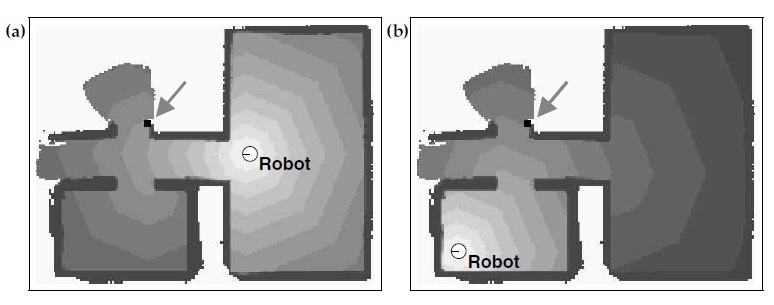
\includegraphics[width=1\linewidth]{179orig}}
	\caption{ ( Рис. 17. Два робота, исследующих окружающую среду. Без координации оба робота могут принять решение о передвижении в одну и ту же точку. На каждом изображении показаны робот, карта и функция ценности. Чёрным квадратом обозначена точка с минимальной стоимостью.) }
	\label{fig:179orig}
\end{figure}

\begin{figure}[H]
	\center{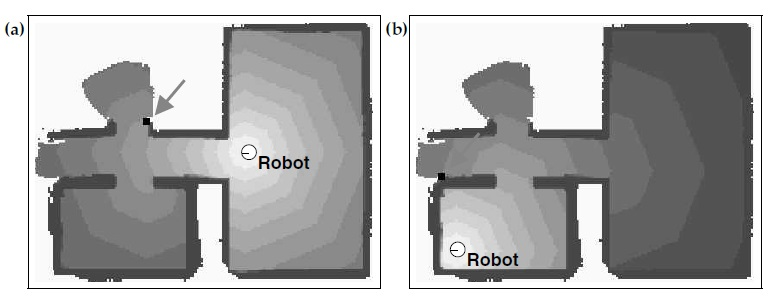
\includegraphics[width=1\linewidth]{1710orig}}
	\caption{ ( Рис. 17.10 Целевые позиции, полученные методом координации. В этом случае целевая точка для второго робота расположена слева в коридоре.) }
	\label{fig:1710orig}
\end{figure}

На Рис. 17.13 показана эффективность этого алгоритма по сравнению с группой роботов, выполняющих алгоритм \textbf{Monte\_Carlo\_exploration} безо всякой координации. По горизонтальной оси показано количество роботов в группе, по вертикальной- количество тактов времени, необходимых для завершения задачи исследования. В этих экспериментах допускалось, что роботы всегда разделяют между собой локальные карты. Кроме того, все роботы  стартовали близко друг от друга. Результат очень нагляден, и, очевидно, некоординированные группы роботов гораздо менее эффективны.

\begin{figure}[H]
	\center{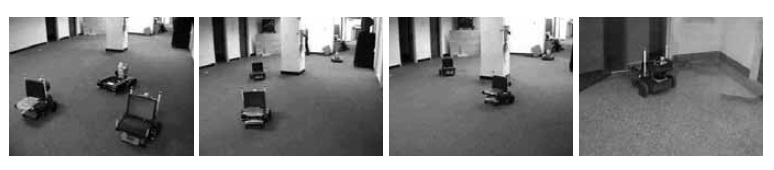
\includegraphics[width=1\linewidth]{1711orig}}
	\caption{ ( Рис. 17.11 Координированное исследование группой мобильных роботов. Роботы распределяются в среде.) }
	\label{fig:1711orig}
\end{figure}

\begin{figure}[H]
	\center{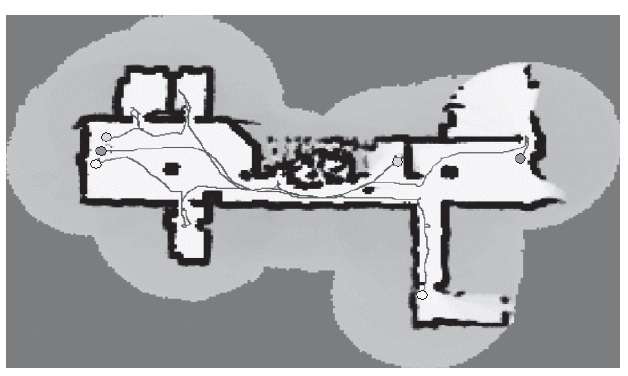
\includegraphics[width=0.85\linewidth]{1712orig}}
	\caption{ ( Карта 17.12 Карта объёмной среды 62$\times$43 м, изученная тремя роботами за 8 минут.) }
	\label{fig:1712orig}
\end{figure}

\begin{figure}[H]
	\center{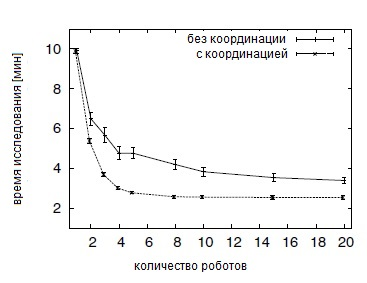
\includegraphics[width=0.6\linewidth]{1713orig}}
	\caption{ ( Рис. 17.13 Время исследования, показанное в имитационном эксперименте, в котором различные группы роботов исследовали среду, показанную выше.) }
	\label{fig:1713orig}
\end{figure}

Пока что обсуждаемые стратегии координации предполагают, что роботы обмениваются картами и знают относительные местоположения. Принимая во внимание неопределённость относительных положений роботов, исследование с помощью нескольких роботов может быть обобщено для случая, когда роботы стартуют из разных, неизвестных заранее положений.

\begin{figure}[H]
	\center{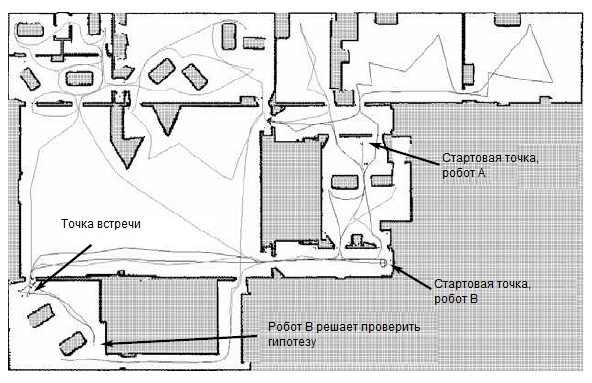
\includegraphics[width=0.95\linewidth]{1714orig}}
	\caption{ ( Рис. 17.14 Координированное исследование при неизвестных начальных положениях. Роботы устанавливают общую систему отсчёта, оценивая и проверяя относительное положение друг друга с помощью метода рандеву. При встрече они обмениваются картами и координатами исследований. Собственность Джонатана Ко и Бенсона Лимкеткай (Jonathan Ko and Benson Limketkai).) }
	\label{fig:1714orig}
\end{figure}

На Рис. 17.14 показан эксперимент исследования, использующий такой обобщенный метод координации. Два робота, A и B, не имеют никакой информации о своём местоположении и выполняют исследование независимо друг от друга. По мере исследования, каждый робот оценивает положение другого робота относительно своей карты, используя модифицированную версию MCL локализации. Выбирая, куда двигаться дальше, оба робота A и B оценивают, что будет «выгоднее» - двинуться в неисследованную зону, или проверить гипотезу о местонахождении другого робота. В какой-то момент времени, робот B принимает решение проверить гипотезу об определении местонахождении робота A. Он посылает роботу A команду остановиться и двигается в предполагаемую точку его местонахождения (помеченную как точка встречи на Рис. 17.14). По прибытии в эту точку, оба робота проверяют наличие друг друга с помощью лазерных датчиков расстояния (роботы помечены светоотражающей лентой). После обнаружения друг друга они объединяют карты и обобщают систему отсчета. С этого момента они исследуют среду с помощью алгоритма \textbf{multi\_robot\_exploration}. Такой метод исследования из неизвестных начальных местоположений можно применять для сценариев с более чем двумя роботами.\\

\textbf{17.5	Исследование для SLAM}\\

В последнем алгоритме этой книги идея жадного исследования применяется к полному алгоритму SLAM. В предыдущих разделах мы всегда подразумевали, что карта или положение робота известны. В SLAM, однако, неизвестно ни то, ни другое. Соответственно, требуется учитывать неопределённость карты и положения робота при выборе способа исследования, поскольку можно получить или потерять информацию об обоих величинах. Очевидно, без знания положения робота интеграция информации датчиков в карту может привести к серьёзным ошибкам. С другой стороны, робот, который стремится только уменьшить неопределённость положения, просто не будет двигаться и никогда не получит информации о среде за пределами действия датчиков.\\

\textbf{17.5.1	Разложение энтропии в SLAM}\\

Ключевой идеей оптимального исследования в SLAM является то, что энтропия апостериорного распределения SLAM может быть \textit{разложена} на две части. Одна часть относится к энтропии апостериорного распределения положения, а вторая – ожидаемой энтропии карты. Таким образом, робот, выполняющий исследование в задаче SLAM, разменивает неопределённость положения робота на неопределённость карты. Действия управления могут уменьшить только одну из двух. При замыкании цикла робот уменьшает неопределённость положения. При перемещении в открытую неисследованную область он, в основном, уменьшает неопределённость карты. Учитывая значения обоих видов неопределённости, робот принимает решение выполнить действие, которое будет в максимальной степени ее уменьшать, поэтому робот иногда будет двигаться на открытое место, а иногда – выполнять локализацию, возвращаясь в уже исследованные области.

Разложение энтропии, фактически, универсально для полной задачи SLAM. Будем считать апостериорное распределение SLAM в виде.\\

(17.17)
$$p(x_{1:t},m|z_{1:t},u_{1:t})$$

Его можно разложить следующим образом:\\

(17.18)
$$p(x_{1:t},m|z_{1:t},u_{1:t})=p(x_{1:t}|z_{1:t},u_{1:t})p(m|x_{1:t},z_{1:t},u_{1:t})$$

Это тривиально и уже приводилось в выражении (13.2) на странице 442 ???. Менее очевидно следствие\\

(17.19)
\begin{equation*}
\begin{split}
H&[p(x_{1:t},m|z_{1:t},u_{1:t})]\\
&=H[p(x_{1:t}|z_{1:t},u_{1:t})]+E[H[p(m|x_{1:t},z_{1:t},u_{1:t})]]
\end{split}
\end{equation*}

где ожидание берётся по апостериорной вероятности $p(x_{1:t}|z_{1:t},u_{1:t})$.

Записав   $p(x, m)$  как сокращённую форму полной апостериорной вероятности  $p(x_{1:t},m|z_{1:t},u_{1:t})$, можно вывести разложение в аддитивном виде:\\

(17.20)
\begin{equation*}
\begin{split}
H(x,m)&=E_{x,m}[-\log p(x,m)]\\
&=E_{x,m}[-\log (p(x)p(m|x))]\\
&=E_{x,m}[-\log p(x)-\log p(m|x)]\\
&=E_{x,m}[-\log p(x)]+E_{x,m}[-\log p(m|x)]\\
&=E_x[-\log p(x)]+\int_{x,m}-p(x,m)\log p(m|x)dx\,dm\\
&=E_x[-\log p(x)]+\int_{x,m}-p(m|x)p(x)\log p(m|x)dx\,dm\\
&=E_x[-\log p(x)]+\int_xp(x)\int_m-p(m|x)\log p(m|x)dx\,dm\\
&=H(x)+\int_xp(x)H(m|x)dx\\
&=H(x)+E_x[H(m|x)]
\end{split}
\end{equation*}

Это преобразование напрямую даст разложение в (17.19). Оно доказывает, что энтропия SLAM – это сумма энтропии пути и ожидаемой энтропии карты.\\

\textbf{17.5.2	Исследование в FastSLAM}\\

Теперь переложим разложение энтропии на алгоритм исследования SLAM. Метод основан на алгоритме FastSLAM, описанном в Главе 13 книги, а именно, FastSLAM на основе сеток в подразделе 13.10. Напомним, что FastSLAM отображает апостериорную вероятность SLAM в виде набора частиц. В каждой частице содержится путь робота. В случае реализации на основе сетки, каждая частица также содержит карту сетки занятости. Это позволяет применить меру энтропии для карт сеток занятости, как было описано в предыдущем разделе.

Алгоритм определения последовательности действий исследования приведён в Таблице 17.3. Он оставляет открытыми рад важных вопросов реализации, поскольку служит только схематической иллюстрацией, но характеризует все основные шаги реальной реализации идеи исследования SLAM.

Алгоритм исследования FastSLAM, в основном, выполняет оценку и проверку. В нем предлагается последовательность действий для исследования, которая, затем, оценивается путём измерения остаточной энтропии. Основываясь на фундаментальных принципах, описанных выше, энтропия вычисляется в виде суммы двух членов. Первое слагаемое соответствует положению робота в конце предлагаемой последовательности исследования, а второе – описывает ожидаемую энтропию карты. Затем алгоритм исследования выполняет выбор действий управления, минимизирующих энтропию.

\begin{table}[H]
\begin{center}
\begin{tabular}{|l|}
\hline
{}\\
1:\textbf{ Algorithm FastSLAM\_exploration}$(Y_t):\qquad\qquad\qquad\qquad\qquad$\\
2:\hspace{5mm}$\textit{инициализировать}\,\,\hat{h}=\infty$\\
3:\hspace{5mm}$\textit{повторять}$\\
4:\hspace{10mm}
$\textit{предложить последовательность действий для исследования}\,\,u_{t+1:T}$\\
5:\hspace{10mm}$\textit{выбрать случайную частицу}\,\,y_t\in Y_t$\\
6:\hspace{10mm}$\textit{для}\,\,\tau=t+1\,\,\textit{до}\,\,T$\\
7:\hspace{15mm}$\textit{извлечь}\,\,x_{\tau}\sim p(x_{\tau}|u_{\tau},x_{\tau-1})$\\
8:\hspace{15mm}$\textit{извлечь}\,\,z_{\tau}\sim p(z_{\tau}|x_{\tau})$\\
9:\hspace{15mm}$\textit{вычислить}\,\,Y_{\tau}=\textbf{FastSLAM}\,(z_{\tau},u_{\tau},Y_{\tau-1})$\\
10:\hspace{9mm}$\textit{endfor}$\\
11:\hspace{9mm}$\textit{обучить гауссову функцию}\,\,\mu_x,\varSigma_x\,\,\textit{для всех частиц положений}\,\,\{x_T^{[k]}\}\in Y_T$\\
12:\hspace{9mm}$h=\frac{1}{2}\log\det(\varSigma_x)$\\
13:\hspace{9mm}$\textit{для частиц}\,\,k=1\,\,\textit{до}\,\,M\,\,\textit{выполнять}$\\
14:\hspace{14mm}$\textit{пусть m - карта}\,\,m_T^{[k]}\,\,\textit{из k-й частицы в}\,\,Y_T$\\
15:\hspace{14mm}$\textit{обновить}\,\,h=h+\frac{1}{M}H[m]$\\
16:\hspace{9mm}$\textit{endfor}$\\
17:\hspace{9mm}$\textit{if}\,\,h<\hat{h}\,\,\textit{then}$\\
18:\hspace{14mm}$\textit{установить}\,\,\hat{h}=h$\\
19:\hspace{14mm}$\textit{установить}\,\,\hat{u}_{t+1:T}=u_{t+1:T}$\\
20:\hspace{9mm}$\textit{endif}$\\
21:\hspace{4mm}$\textit{до сходимости}$\\
22:\hspace{4mm}$\textit{return}\,\,\hat{u}_{t+1:T}$\\
{}\\
\hline
\end{tabular}
\caption{(Таблица 17.3 Алгоритм исследования для версии FastSLAM на основе сеток. На вход принимается набор частиц $Y_t$. Каждая частица $y_t^{[k]}$  содержит выборку пути робота $x_{1:t}^{[k]}$  и связанную карту сетки занятости $m^{[k]}$. На выходе создаётся путь исследования, выраженный в виде команд относительного движения. )}
\end{center}
\end{table}

Более детально, алгоритм \textbf{FastSLAM\_exploration} принимает на вход набор частиц, а возвращает предполагаемую последовательность действий управления для исследования. В строке 4 Таблицы 17.3 предложена потенциальная последовательность управления. Проверка последовательности управления выполняется в строках с 5 по 16. Она состоит из трёх частей. Во-первых, робот смоделирован на основе случайной частицы в наборе частиц. В этом моделировании использована стохастическая модель робота и среды. Результатом является последовательность наборов частиц по всему пути до конца управляемой траектории. Моделирование выполняется в строках с 5 по 9.

Вслед за этим вычисляется энтропия финального набора частиц. С помощью математического разложения, приведённого в Выражении 17.19, энтропия разбивается на два слагаемых: первое относится к оценке энтропии положения робота в момент $T$, а второе – к ожидаемой энтропии карты. Первое слагаемое вычисляется в строках 11 12. Его правильность следует из правильности выведения энтропии гауссовой функции, приведённой в Таблице. 17.4.

\begin{table}[H]
\begin{center}
\begin{tabular}{|l|}
\hline
{}\\
\text{\textbf{Лемма}.  \textit{Энтропия многомерного гауссиана} с $d$ измерениями и}\\
\text{ $\varSigma$ задана в виде}\\
$H=\frac{d}{2}(1+\log2\pi)+\frac{1}{2}\log\det(\varSigma)$\\
\text{\textbf{Доказательство}. Для}\\
$p(x)=(2\pi)^{-\frac{d}{2}}\det(\varSigma)^{-\frac{1}{2}}\exp\{-\frac{1}{2}x^T\varSigma^{-1}x+x^T\varSigma^{-1}\mu-\frac{1}{2}\mu^T\varSigma^{-1}\mu\}$\\
\text{получим}\\
$H_p[x]=E[-\log p(x)]$\\
$\,\,\,\,\,=\frac{1}{2}(d\log2\pi+\log\det(\varSigma)+E[x^T\varSigma^{-1}x]-2E[x^T]\varSigma^{-1}\mu+\mu^T\varSigma^{-1}\mu)$\\
\text{Здесь}$E[x^T]=\mu^T$,\,\text{и}$\,\,E[x^T\,\,\varSigma^{-1}\,\,x]\,\,$\text{разрешаются в следующем виде}\\
\text{(где “·” обозначает умножение)}\\
$E[x^T\,\,\varSigma^{-1}\,\,x]=E[x\,\,x^T\,\cdot\,\varSigma^{-1}]$\\
$\hspace{21mm}=E[x\,\,x^T]\,\cdot\,\varSigma^{-1}$\\
$\hspace{21mm}=\mu\,\mu^T\,\cdot\,\varSigma^{-1}+\varSigma\,\cdot\,\varSigma^{-1}$\\
$\hspace{21mm}=\mu^T\varSigma^{-1}\mu+d$\\
\text{Из этого следует, что}\\
$H_p[x]=\frac{1}{2}(d\log2\pi+\log\det(\varSigma)+\mu^T\varSigma^{-1}\mu+d-2\mu^T\varSigma^{-1}\mu+\mu^T\varSigma^{-1}\mu)$\\
$\hspace{9mm}=\frac{d}{2}(1+\log2\pi)+\frac{1}{2}\log\det(\varSigma)$\\
{}\\
\hline
\end{tabular}
\caption{(Таблица 17.4   Энтропия многомерного гауссиана)}
\end{center}
\end{table}

Второй член, выражающий энтропию, вычисляется в строках с 13 по 16. Заметим, что вычисление включает энтропию карты $m$ и для карт сетки занятости выполняется аналогично обсуждаемому в предыдущем разделе. В строках с 13 по 16 вычисляется средняя энтропия карты в виде среднего значения по всем частицам в момент времени $T$. Результатом является значение $h$, измеряющее ожидаемую энтропию в момент времени $T$, зависящий от предполагаемой последовательности управления. Затем в строках с 17 по 20 выбирается последовательность действий, минимизирующая ожидаемую энтропию, которая возвращается в строке 22.

Заметим, что в алгоритме для вычисления энтропии апостериорной вероятности по траекториям в строке 11 используется аппроксимация. Вместо  выражения гауссиана по всем траекториям частиц $y_T^{[k]}$, вычисление производится на основании последних положений $x_T^{[k]}$.
Это приближение хорошо работает на практике, и напоминает уже приведённый вид аппроксимации действия исследования.

В итоге, алгоритм исследования FastSLAM, в основном, является обобщением исследовательского алгоритма методом Монте-Карло, приведённого в Таблице 17.1, с двумя отличиями. Во-первых, он применяется к целым последовательностям управляющих воздействий, а не только к одному действию. Во-вторых, что более важно, алгоритм исследования FastSLAM вычисляет два типа энтропии, один для пути робота и один для карты.\\

\textbf{17.5.3	Эмпирическое определение}\\

Алгоритм исследования приводит к соответствующему поведению робота, особенно в циклических средах. На Рис. 17.15 показана ситуация, когда робот исследует \textit{циклическую среду}, в которой имеется \textit{петля}. Робот начинает в правом нижнем углу цикла, помеченной “Начало”. На такте времени 35, предпринимаемые роботом действия снова приводят его на стартовую точку, рядом с неизвестной зоной слева от маркера. Общий прирост информации от возвращения на старт выше, чем продвижение вглубь неизвестной области, поскольку, вдобавок к новой информации на карте, будет уменьшена неопределённость положения. Поэтому робот, выполняющий активное исследование, решает замкнуть цикл и двигаться по уже обследованной территории.

На Рис. 17.16 более подробно показан компромисс между стоимостью и наградой. На ней показано 8 различных действий. Полезность действия 1 наивысшая и существенно превышает полезность действия 4 (и любых других действий без замыкания цикла).

На такте времени 45 робот замыкает цикл, как показано на Рис. 17.15. В этой точке неопределённость положения минимальна, и неопределённость карты начинает преобладать. В результате, действие замыкания цикла уже не выглядит привлекательным. В момент времени 88 робот выбирает исследования большой открытой области, к которой он и следует, что видно из Рис. 17.15.

На Рис. 17.17 показано изменение общей энтропии в эксперименте со временем. До такта времени 30, уменьшение неопределённости карты компенсировало увеличение неопределённости по траектории робота и энтропия оставалась более-менее постоянной. Хотя действие замыкания цикла уменьшает энтропию гипотезы по траектории робота, изменения неопределённости карты относительно мало. Это приводит к уменьшению общей энтропии. По мере того, как робот учитывает измерения, покрывающие доселе неизвестные области горизонтального коридора, изменения неопределённости карты и положения робота компенсируют друг друга. Падение общей энтропии около такта времени 90 вызвано наблюдениями в широкой части коридора. Это происходит потому, что карты сеток занятости уменьшают неопределённость карты, учитывая проход сканирования дальности, что почти линейно зависит от размера неизвестной зоны, покрываемой проходом сканирования.

Сложная взаимосвязь между неопределённостью карты и пути, и соответствующие понятия прироста информации играют важную роль в алгоритме исследования. Робот выбирает локализацию, когда это предпочтительно, но иногда движется в неизвестную область. 

\begin{figure}[H]
	\center{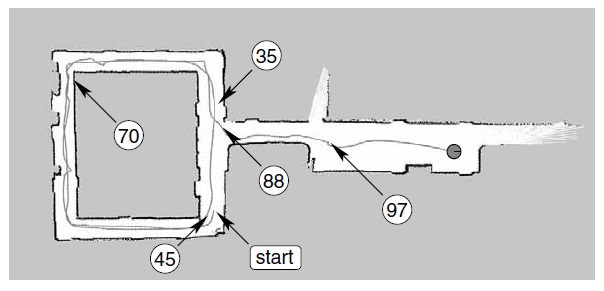
\includegraphics[width=1\linewidth]{1715orig}}
	\caption{ ( Рис. 17.15 Мобильный робот исследует циклическую среду. Робот начинает в правом нижнем углу цикла. После прохода по всему циклу, он решает повторить траекторию, чтобы уменьшить неопределённость, а затем продолжает исследование коридора. Рисунок принадлежит Сирилу Стачнису, университет Фрайбурга (Cyrill Stachniss, University of Freiburg).) }
	\label{fig:1715orig}
\end{figure}

\begin{figure}[H]
	\center{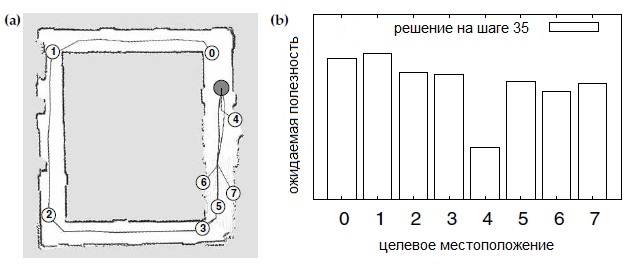
\includegraphics[width=1\linewidth]{1716orig}}
	\caption{ ( Рис. 17.16 В этой ситуации робот определяет ожидаемую полезность действий.  действия исследования, рассматриваемые роботом(a), и  ожидаемая полезность каждого действия (b). Действие 1 выбирается потому, что оно максимизирует ожидаемую полезность. Рисунок принадлежит Сирилу Стачнису, университет Фрайбурга (Cyrill Stachniss, University of Freiburg). ) }
	\label{fig:1716orig}
\end{figure}

\begin{figure}[H]
	\center{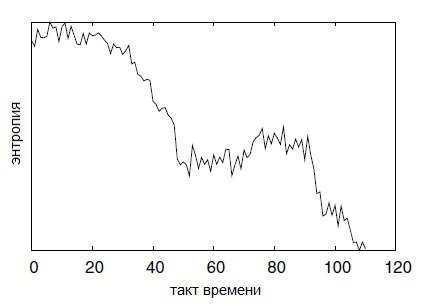
\includegraphics[width=0.6\linewidth]{1717orig}}
	\caption{ ( Рис. 17.17 Изменение энтропии в ходе исследовательского эксперимента, показанного на Рис. 17.15. Рисунок принадлежит Сирилу Стачнису, университет Фрайбурга (Cyrill Stachniss, University of Freiburg).) }
	\label{fig:1717orig}
\end{figure}

\textbf{17.6	Выводы}\\

В этой главе мы узнали об исследованиях с помощью роботов. Все представленные в главе алгоритмы преследуют единственную цель – максимизировать информацию, получаемую роботом. Распределяя действия управления так, чтобы они максимизировали прирост информации, робот способен эффективно выполнять задачи исследования.

Эта идея была использована для решения ряда задач исследования:\\

•	В активной локализации робот стремится максимизировать осведомлённость о своём положении на известной карте. Был выведен алгоритм, вычисляющий ожидаемый прирост информации для перемещения в любое из возможных положений робота. В нём устанавливается компромисс между перемещением в точку, дающую максимальный прирост информации и стоимостью такого перемещения. Результирующий алгоритм хорошо выполняет отбор местоположений на основе прироста информации.\\

•	В исследовании для построения карт робот знает своё положение с самого начала, но должен собирать данные об окружающей среде. После анализа идеи карты сетки занятости было замечено, что прирост информации можно вычислить отдельно для каждой ячейки на карте. После сравнения нескольких разных методов вычисления прироста информации была показана пригодность для практического использования даже самых простых методов, например, энтропии. Затем был выведен динамический алгоритм программирования перемещения в ближайшую точку с наилучшим балансом между приростом информации и стоимостью перемещения.\\

•	Мы дополнили метод исследования на основе прироста информации для случая группы роботов. Это обобщение оказалось удивительно простым, поскольку очевидная модификация парадигмы динамического программирования сделала возможным вычисление стоимости перемещения в любое местоположение, сравнительно с приростом информации. На основании сравнения стоимости и прироста информации для разных местоположений, несколько роботов могут координировать цели для минимизации общего времени исследования.\\

•	Наконец, обсуждались методы исследования для полной задачи SLAM, когда и положение робота, и карта окружающей среды неизвестны. Рассмотренный метод основан на разбиении энтропии на два компонента, первый из которых выражает неопределённость пути, а второй – неопределённость карты (усреднённую по всем возможным путям). Это соображение позволило создать алгоритм генерации и проверки для задачи исследования, в котором генерируются управляющие последовательности и вычисляются будущие оценки, позволяющие найти баланс между неопределённостями пути и карты при оценке последовательностей управления. Результатом стал метод исследования, в котором робот иногда двигается в неисследованные области для уменьшения неопределённости карты, а, иногда – возвращается на уже посещённые участки для улучшения оценок положения.\\

Большинство методов в этой главе – жадные, поскольку робот рассматривает единственный вариант выбора управляющего действия. Эта жадность стала результатом огромного коэффициента ветвления в большинстве задач исследования, что делает планирование на несколько шагов вперёд неприменимым. Однако, выбор правильного действия исследования потребовал некоторых размышлений.

Алгоритмы в этой главе рассматривают в качестве действия исследования робота перемещение в любую точку локальной координатной системы. Поэтому рассматриваемый базовый блок движения существенно превосходит общий блок движения, определённый в Главе 5. Но именно такое определение действия делает кажущиеся простыми методы применимыми для сложных многоэтапных задач исследования с помощью роботов.

Было замечено, что исследование можно сформулировать в виде общей задачи POMDP, используя функцию дохода, которая награждает за прирост информации. Однако, методы POMDP лучше использовать при малом коэффициенте ветвления и ограниченном числе возможных наблюдений. Задачи исследования характеризуются огромными пространствами состояний и наблюдений. В силу этого их лучше всего решать с помощью жадных методов, которые напрямую максимизируют прирост информации. \\

\textbf{17.7	Библиографические примечания.}\\

Исследование было основной областью разработки робототехнических систем, которые использовались в таких областях, как исследование вулканов (Bares and Wettergreen 1999; Wettergreen et al. 1999), лун и планет (Gat et al. 1994; Höllerer et al. 1999; Krotkov et al. 1999; Matthies et al. 1995; Li et al. 2000), поиск и спасение (Murphy 2004), составление карт заброшенных шахт (Madhavan et al. 1999; Thrun et al. 2004c; Baker et al. 2004), поиск метеоритов в Антарктике (Urmson et al. 2001; Apostolopoulos et al. 2001), исследование пустынь (Bapna et al. 1998) а также подводные исследования (Ballard 1987; Sandwell 1997; Smith and Dunn 1995; Whitcomb 2000).

Литература по разработке алгоритмов по исследованию с помощью роботов уходит корнями в различные области теории информации и принятия решений, описанных в двух предыдущих главах. Одним из ранних методов исследования с помощью роботов является алгоритм, описанный Куперсом и Буном (Kuipers and Byun, 1990, 1991), а также Пирсом и Куперсом (Pierce and Kuipers, 1994). В этом методе робот идентифицирует так называемые локально различимые места, что позволяет ему отличать уже посещённые и ещё неисследованные зоны. Похожая базовая работа принадлежит Дудеку (Dudek et al., 1991), который разработал стратегию исследования неизвестной среды наподобие графа. Эти алгоритмы не учитывали расстояний и были специально разработаны для роботов с ограниченными способностями к восприятию.

Ранний метод исследования для изучения топологических карт мобильными роботами был предложен Кенигом и Симмонсом (Koenig and Simmons, 1993). Идея активного исследования для карт сеток занятости на основе динамического программирования восходит к работам Моравица и Труна (Moravec, 1988 and Thrun, 1993). Тейлор и Кригман (Tailor and Kriegman, 1993) описали метод посещения всех ориентиров в среде для построения карты на основе признаков. В этой системе робот сохраняет список всех не посещённых ориентиров среды. Идею максимизации информации в исследовании с помощью статистической формулировки можно найти в работе Келблинга (Kaelbling et al., 1996). Ямагучи (Yamauchi et al., 1999) представил метод исследования на основе границ, где границы между исследованными и неисследованными областями специально использовались для управления действиями робота. Позже Гонсалес-Банос и Латомбе (González-Baños and Latombe, 2001) предложили стратегию исследования, где для определения следующего действия учитывался размер невидимой зоны, которая может стать видимой с нескольких возможных точек наблюдения. Похожие методы исследования стали популярными в области моделирования трёхмерных объектов. Например, Уайти и Ферри (Whaite and Ferrie, 1997) изучили задачу сканирования объектов и учёта неопределённости параметров модели при определении следующей лучшей точки зрения.

Метод исследования также был обобщён для групп роботов, действующих совместно. Бургард (Burgard et al., 2000, 2004), и Симмонс (Simmons et al., 2000a) расширили жадную концепцию исследования для групп роботов, которые выполняли исследование совместно, пытаясь максимизировать информацию карты. Этот подход похож на метод инкрементного размещения, введённый Говардом (Howard et al., 2002) и на алгоритм, предложенный Страупом (Stroupe, 2004). Методы на основе рынка для координированного поиска были исследованы Злотом (Zlot et al., 2002). Диас (Dias et al., 2004) анализировал потенциальные отказы при координации нескольких роботов, предложив улучшенный алгоритм. Метод для работы с гетерогенными группами роботов был представлен Сингхом и Фуджимура (Singh and Fujimura, 1993). Обобщение для координированного исследования из нескольких, неизвестных стартовых локаций, было представлено Ко (Ko et al., 2003) и тщательно проверено Конолигом (Konolige et al., 2005). Этот метод использует структурную оценку среды вместе с модифицированной версией локализации MCL для оценки относительных местоположений робота (Fox et al. 2005). В работе Реклейтиса (Rekleitis et al., 2001b), авторы предложили метод исследования, в котором один робот наблюдал местоположение второго, выполняющего исследование, уменьшая, таким образом, его неопределённость местоположения. Некоторые из экспериментов с несколькими роботами, представленные в этой главе, были впервые описаны Труном (Thrun, 2001).\\

ЗАДАЧА ПОКРЫТИЯ\\

В некоторых публикациях задача исследования карты изучалась как \textit{задача покрытия}, освещая проблему проектирования алгоритма для покрытия неизвестной среды. В новой работе Чосета (Choset, 2001) дан подробный обзор в этой области. Более новые методы (Acar and Choset 2002; Acar et al. 2003) используют для решения этой проблемы статистику, с алгоритмами не слишком отличными от представленных в книге.

В контексте SLAM несколько авторов вывели методы исследования, совместно выполняющие оптимизацию покрытия карты и активную локализацию. Макаренко (Makarenko et al., 2002) описал метод, определяющий необходимые действия на основе ожидаемого прироста информации, полученного при повторном наблюдении ориентиров (для более точного определения местоположения или положения робота) и при исследовании неизвестных мест. Похожим образом, Ньюман (Newman et al., 2003) описал метод исследования в контексте фреймворка  Atlas (Bosse et al. 2003) для эффективного SLAM. В этом методе робот строит структуру наподобие графа для хранения информации об уже посещённых местах. Сим (Sim et al., 2004) специально обратил внимание на задачу планирования траектории в SLAM. В нем учитывался специальный параметрический класс политик спиральных траекторий в контексте метода на основе EKF для задачи SLAM. Метод исследования FastSLAM, описанный в этой главе, принадлежит Стачнису и Бургарду  (Stachniss and Burgard, 2003, 2004). Исследование на базе SLAM, где робот выкладывает маркеры, чтобы облегчить локализацию, описана Баталиным и Сухатме (Batalin and Sukhatme,  2003).

Анализ эффективности методов исследования с помощью роботов также был объектом значительного интереса. Несколько авторов предоставили математический и эмпирический анализ сложности разных методов исследования (Albers and Henzinger 2000; Deng and Papadimitriou 1998; Koenig and Tovey 2003; Lumelsky et al. 1990; Rao et al. 1993). Например, Ли и Рис (Lee and Recce, 1997) представили экспериментальное исследование, в котором сравнили эффективность различных стратегий исследования для одиночных роботов.

Описанный в книге метод активной локализации для мобильных роботов был впервые опубликован в работах Бургарда (Burgard et al., 1997) и Фокса (Fox et al., 1998). Чуть позже, Янсфельт и Кристенсен (Jensfelt and Christensen, 2001a) представили систему на основе смеси гауссиан для представления апостериорного положения робота и описали способ выполнения активной локализации на основе этого представления. Задача активной локализации была теоретически изучена, например, Келблингом (Kleinberg, 1994) для случая идеальных датчиков.

Несколько авторов разработали методы исследования для динамических сред. Особенный интерес представляют игры в преследование, описанные в обширной литературе по дифференциальным играм (Isaacs 1965; Bardi et al. 1999). Методы ухода от преследования в мобильной робототехнике принадлежат ЛаВалли (LaValle et al., 1997) и Гуйбасу (Guibas et al., 1999), и были недавно расширены Герки (Gerkey et al., 2004).

Наконец, исследование активно изучалось в теории автоматов. Парадигма последовательного принятия решений, в которой агент получает награду в ходе экспериментов изначально изучалась в контексте простых конечных автоматов, известных, как бандиты, см. Фельдман (Feldman, 1962), Берри и Фристедт (Berry and Fristedt, 1985), Роббинс (Robbins, 1952). Методы изучения структуры конечных автоматов восходят к работам Ривеста и Шапире (Rivest and Schapire, 1987a,b) а Мозер и Бахра (Mozer and Bachrach, 1989) разработали методы генерации последовательности проверок, различающие различные состояния в конечных автоматах. Границы сложности на основе состояний для исследуемых детерминированных сред были выведены Кенигом и Симмонсом (Koenig and Simmons, 1993) и Труном (Thrun, 1992), а позже – обобщены для стохастических сред Кирнсом и Сингхом (Kearns and Singh, 2003).\\

\textbf{17.8	Упражнения}\\

1.	Пусть дан робот, действующий в треугольной среде с тремя типами ориентиров:

\begin{figure}[H]
	\center{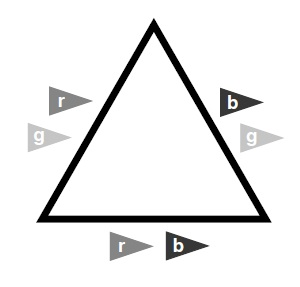
\includegraphics[width=0.4\linewidth]{17treug}}
	\label{fig:17treug}
\end{figure}

Каждое местоположение имеет два разных ориентира, отличающихся по цвету. Допустим, каждый раунд робот может определить наличие только одного типа ориентиров: или обозначенного “r”, или “g”, или “b”. Допустим, робот в начале выстреливает детектор ориентиров “b” и двигается по часовой стрелке до следующей стороны. Какой детектор оптимально использовать следующим? Как изменится ответ, если робот не двигается, или двигается против часовой стрелки до следующей стороны?\\

2.	Допустим, дано $K$ однонаправленных роботов, каждый из которых в этом упражнении может двигаться и выполнять измерения в любое время. В этом упражнении хотелось бы увидеть каждый видимый ориентир только единожды. О преимуществах повторного ориентира пока беспокоиться не нужно.\\

В тексте отмечалось, что использование нескольких роботов может ускорить исследование больше, чем на линейный коэффициент количества роботов (то есть $K$ могут быть в более чем $K$ раз быстрее, чем 1 робот).\\

(a)	Насколько быстрее группа из $K$ будет быстрее по сравнению с одним роботом?\\

(b)	Дать пример среды, максимизирующей ускорение исследования для $K$ = 4 роботов, и обсудить стратегию исследования, которая даст такое ускорение.\\

3.	Допустим, выполняется преследование нарушителя в ограниченной известной среде. Можно ли изобразить среду, где $K$ роботов могут преуспеть в обнаружении нарушителя за конечное время, но $K-1$ роботов уже не могут. Нарисовать среду для $K = 2$, $K = 3$, и $K = 4$ роботов. Заметим, что результат не даёт никаких допущений относительно стратегии движения нарушителя кроме одного – если нарушитель попадает в поле зрения, он замечен.\\

ЗАДАЧА БАНДИТА\\

4. Очень упрощенная задача исследования известна как задача $K$-\textit{рукого бандита}. В ней перед вами игральный автомат с $K$ ручками. Рывок каждой ручки даёт награду \$1 с вероятностью $p_K$, где $p_K$ фиксирована, но неизвестна. Заданием является определение ручек, игра на которых принесёт максимальную награду.\\

(a)	Доказать, что жадная стратегия исследования может быть неоптимальной, где «жадная» определяется как выбор действия относительно функции оценки максимального правдоподобия вероятностей $p_k$. (После $n$ игр на ручке $k$, оценка максимального правдоподобия $p_k$ задана как $n_k/n$, где $n_k$  - количество раз, когда была получена награда \$1).\\

(b)	Доказать, что оптимальная стратегия исследования никогда не будет исключать ни одну из ручек.\\

(c)	Реализовать алгоритм $K$-рукого бандита для $K = 2$, с обоими вероятностями $p_1$ и $p_2$, выбранными равномерно на интервале $[0; 1]$. Реализовать самую лучшую стратегию, которую удастся найти. Стратегия исследования может зависеть только от переменных $n_i$ для $i = 1, 2$. Объяснить стратегию, и измерить общий доход для 1000 игр из 100 шагов каждая.\\

5.	В подразделе 17.4 мы эмпирически сравнили два метода вычисления прироста информации для ячейки сети: энтропию и ожидаемый прирост энтропии. Дать математическую границу ошибки между двумя величинами при допущениях, указанных в главе. Для каких значений занятости карты эта ошибка будет максимальна? Для каких значений она будет минимальна?\\

6.	В тексте мы столкнулись с энтропией в виде гауссовой функции. Требуется вычислить ожидаемый прирост информации для простого обновления гауссиана. Допустим, оценивается неизвестная переменная состояния $x$, а текущие оценки максимального правдоподобия $\mu$ и $\varSigma$. Допустим, что датчик может измерить $x$, но измерение будет повреждено гауссовым шумом с ковариацией $Q$. Дать выражение для ожидаемого прироста информации через выполнение измерений. \textit{Подсказка: Нужно сосредоточиться на ковариации, а не на математическом ожидании.}\\



 
\end{document}